\documentclass[11pt,a4paper]{article}

% Packages
\usepackage[utf8]{inputenc}
\usepackage[T1]{fontenc}
\usepackage{geometry}
\usepackage{graphicx}
\usepackage{booktabs}
\usepackage{longtable}
\usepackage{array}
\usepackage{multirow}
\usepackage{hyperref}
\usepackage{amsmath}
\usepackage{amssymb}
\usepackage{tikz}
\usepackage{float}
\usepackage{listings}
\usepackage{xcolor}
\usepackage{caption}
\usepackage{subcaption}
\usepackage{enumitem}
\usepackage{natbib}

% Page geometry
\geometry{margin=2.5cm}

% TikZ libraries
\usetikzlibrary{shapes.geometric, arrows.meta, positioning, fit, backgrounds, calc}

% Code listing style
\lstset{
    basicstyle=\ttfamily\small,
    breaklines=true,
    frame=single,
    backgroundcolor=\color{gray!10},
    keywordstyle=\color{blue},
    commentstyle=\color{green!60!black},
    stringstyle=\color{orange},
    showstringspaces=false
}

% Hyperref setup
\hypersetup{
    colorlinks=true,
    linkcolor=blue,
    filecolor=magenta,
    urlcolor=cyan,
    citecolor=blue
}

% Title information
\title{\textbf{Nuclear Energy Projection and Avoided Emissions Analysis:\\
An Automated Data Science Pipeline for Climate Transition Risk Assessment}}

\author{
    Climate Data Science Research Project\\
    \textit{Research and Emerging Topics}\\
    Academic Year 2025-2026
}

\date{\today}

\begin{document}

\maketitle

\begin{abstract}
This technical report presents the development and deployment of an automated, reproducible data science pipeline for nuclear energy projection and avoided emissions analysis under IEA Net Zero 2050 scenarios. The pipeline processes data from the Global Nuclear Power Tracker (1,749 plants across 61 countries) and IEA scenario targets to project regional and global nuclear generation from 2025 to 2050. The system implements both deterministic and probabilistic (Monte Carlo) modeling approaches with uncertainty quantification, enabling scenario-based analysis of nuclear energy's contribution to climate mitigation. Key outputs include generation projections reaching 5,000--7,000 TWh globally by 2050, gap analysis against IEA targets, and avoided emissions calculations of 30--50 GtCO$_2$ cumulative (2025--2050). The pipeline is deployed as an interactive Streamlit dashboard and is fully reproducible via version-controlled code with modular architecture.
\end{abstract}

\tableofcontents
\newpage

%==============================================================================
\section{Introduction}
%==============================================================================

Climate transition risk analysis requires robust, automated systems capable of projecting energy generation under multiple scenarios while quantifying uncertainty. Nuclear energy, as a low-carbon electricity source, plays a critical role in decarbonization pathways outlined by the International Energy Agency (IEA) Net Zero 2050 scenario.

This project develops an end-to-end data science pipeline that:
\begin{itemize}[noitemsep]
    \item Ingests and processes global nuclear plant data from authoritative sources
    \item Engineers features for capacity factor estimation and generation calculation
    \item Projects regional and global nuclear generation to 2050 under multiple scenarios
    \item Compares projections against IEA Net Zero targets to identify gaps
    \item Calculates avoided CO$_2$ emissions from nuclear replacing fossil fuel generation
    \item Deploys results via an interactive dashboard for stakeholder communication
\end{itemize}

The pipeline is designed with reproducibility, modularity, and automation as core principles, enabling scalable climate analytics for research and policy applications.

%==============================================================================
\section{Technical Architecture}
%==============================================================================

\subsection{System Overview}

The pipeline follows a modular architecture with five sequential processing stages, each implemented as an independent Python class. Figure~\ref{fig:architecture} illustrates the complete system architecture.

\begin{figure}[H]
\centering
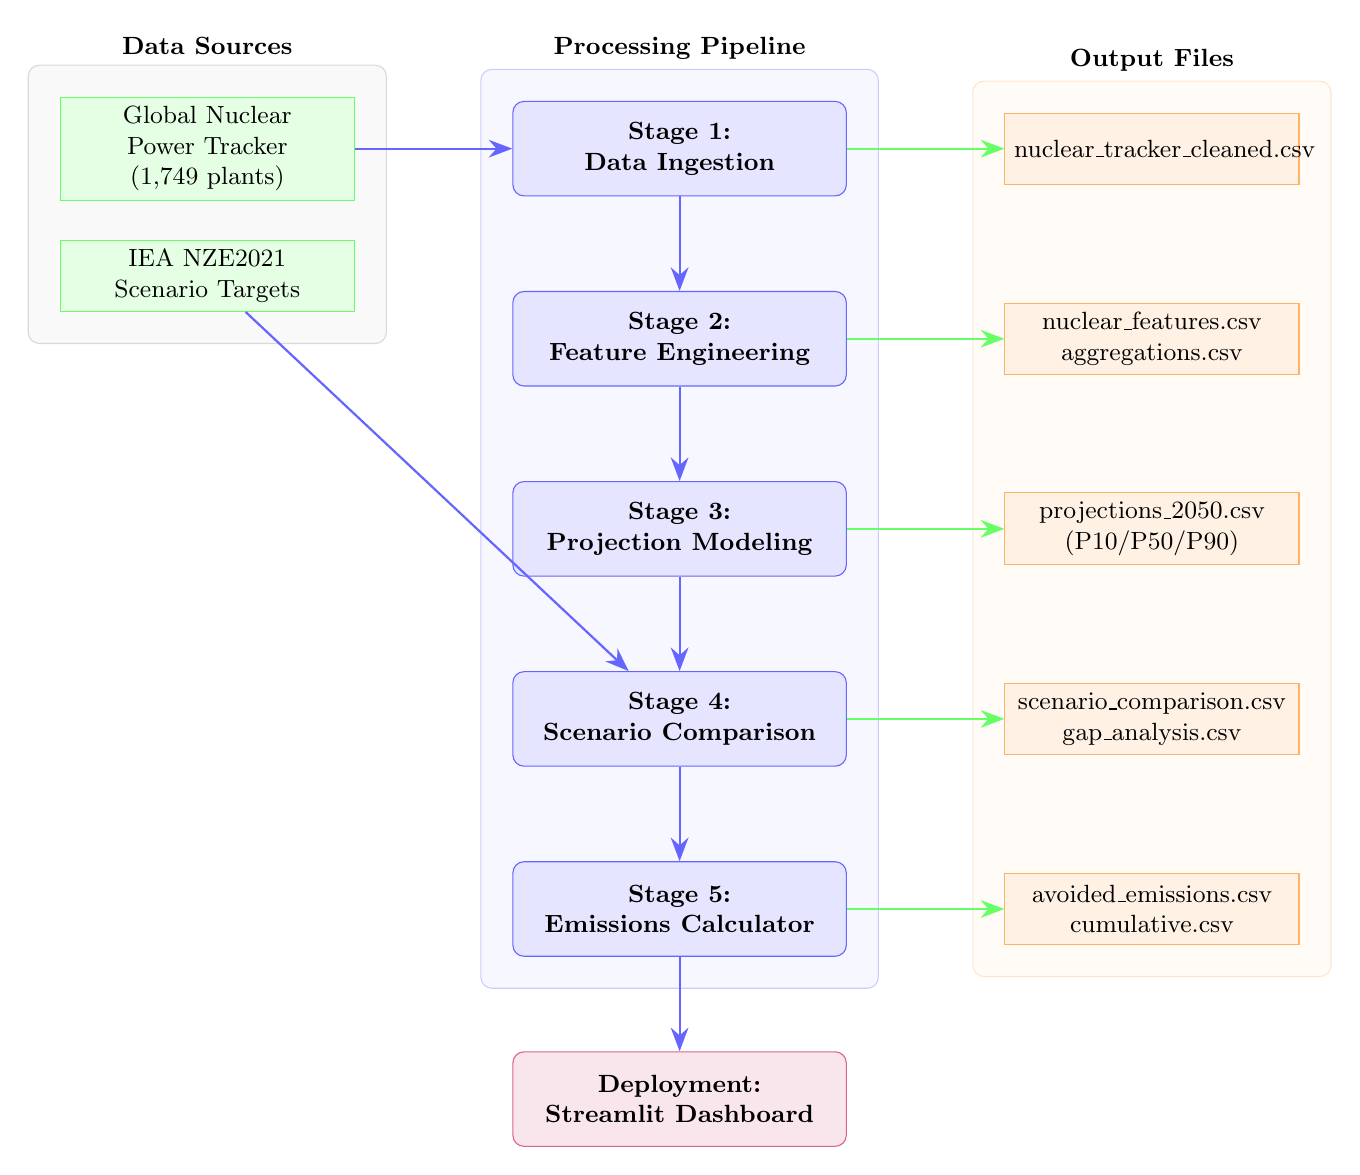
\begin{tikzpicture}[
    node distance=1.2cm,
    stage/.style={rectangle, draw=blue!60, fill=blue!10, text width=4cm, minimum height=1.2cm, align=center, rounded corners, font=\small\bfseries},
    data/.style={rectangle, draw=green!60, fill=green!10, text width=3.5cm, minimum height=0.9cm, align=center, font=\small},
    output/.style={rectangle, draw=orange!60, fill=orange!10, text width=3.5cm, minimum height=0.9cm, align=center, font=\small},
    arrow/.style={-{Stealth[length=3mm]}, thick, blue!60}
]

% Data Sources (left column)
\node[data] (raw1) {Global Nuclear Power Tracker\\(1,749 plants)};
\node[data, below=0.5cm of raw1] (raw2) {IEA NZE2021\\Scenario Targets};

% Pipeline stages (center column)
\node[stage, right=2cm of raw1] (ingest) {Stage 1:\\Data Ingestion};
\node[stage, below=of ingest] (feature) {Stage 2:\\Feature Engineering};
\node[stage, below=of feature] (project) {Stage 3:\\Projection Modeling};
\node[stage, below=of project] (scenario) {Stage 4:\\Scenario Comparison};
\node[stage, below=of scenario] (emissions) {Stage 5:\\Emissions Calculator};

% Output files (right column)
\node[output, right=2cm of ingest] (out1) {nuclear\_tracker\_cleaned.csv};
\node[output, right=2cm of feature] (out2) {nuclear\_features.csv\\aggregations.csv};
\node[output, right=2cm of project] (out3) {projections\_2050.csv\\(P10/P50/P90)};
\node[output, right=2cm of scenario] (out4) {scenario\_comparison.csv\\gap\_analysis.csv};
\node[output, right=2cm of emissions] (out5) {avoided\_emissions.csv\\cumulative.csv};

% Deployment
\node[stage, below=of emissions, fill=purple!10, draw=purple!60] (deploy) {Deployment:\\Streamlit Dashboard};

% Arrows - data to pipeline
\draw[arrow] (raw1) -- (ingest);
\draw[arrow] (raw2) -- (scenario);

% Arrows - pipeline flow
\draw[arrow] (ingest) -- (feature);
\draw[arrow] (feature) -- (project);
\draw[arrow] (project) -- (scenario);
\draw[arrow] (scenario) -- (emissions);
\draw[arrow] (emissions) -- (deploy);

% Arrows - outputs
\draw[arrow, green!60] (ingest) -- (out1);
\draw[arrow, green!60] (feature) -- (out2);
\draw[arrow, green!60] (project) -- (out3);
\draw[arrow, green!60] (scenario) -- (out4);
\draw[arrow, green!60] (emissions) -- (out5);

% Background boxes
\begin{scope}[on background layer]
    \node[fit=(raw1)(raw2), fill=gray!5, draw=gray!30, rounded corners, inner sep=0.4cm, label={[font=\small\bfseries]above:Data Sources}] {};
    \node[fit=(ingest)(emissions), fill=blue!3, draw=blue!20, rounded corners, inner sep=0.4cm, label={[font=\small\bfseries]above:Processing Pipeline}] {};
    \node[fit=(out1)(out5), fill=orange!3, draw=orange!20, rounded corners, inner sep=0.4cm, label={[font=\small\bfseries]above:Output Files}] {};
\end{scope}

\end{tikzpicture}
\caption{System Architecture: End-to-end data pipeline from ingestion to deployment}
\label{fig:architecture}
\end{figure}

\subsection{Directory Structure}

The project follows a standardized data science project structure:

\begin{lstlisting}[language=bash, caption={Project Directory Structure}]
researchhamada/
|-- data/
|   |-- raw/                    # Original source data (immutable)
|   |-- processed/              # Pipeline outputs (17 CSV files)
|   +-- external/               # External documentation
|-- src/                        # Core pipeline modules
|   |-- data_ingestion.py       # NuclearDataLoader class
|   |-- feature_engineering.py  # NuclearFeatureEngineer class
|   |-- projection_model.py     # NuclearProjectionModel (v1)
|   |-- projection_model_v2.py  # EnhancedNuclearProjectionModel (v2)
|   |-- scenario_comparison.py  # ScenarioComparison class
|   +-- emissions_calculator.py # EmissionsCalculator class
|-- notebooks/
|   |-- 01_exploratory_analysis_executed.ipynb
|   +-- 02_statistical_analysis.ipynb
|-- outputs/
|   |-- figures/                # Generated visualizations
|   +-- results/                # Statistical summaries
|-- logs/                       # Pipeline execution logs
|-- pipeline.py                 # Main orchestrator
|-- app.py                      # Streamlit dashboard
|-- requirements.txt            # Python dependencies
+-- pyproject.toml              # Project configuration
\end{lstlisting}

\subsection{Technology Stack}

Table~\ref{tab:tech-stack} summarizes the technologies and frameworks used in the pipeline.

\begin{table}[H]
\centering
\caption{Technology Stack}
\label{tab:tech-stack}
\begin{tabular}{@{}lll@{}}
\toprule
\textbf{Category} & \textbf{Technology} & \textbf{Purpose} \\
\midrule
Programming Language & Python 3.11+ & Core development \\
Data Processing & pandas, numpy, openpyxl & Data manipulation, Excel I/O \\
Statistical Analysis & scipy, statsmodels & Hypothesis testing, regression \\
Machine Learning & scikit-learn & PCA, preprocessing \\
Visualization & matplotlib, seaborn, plotly & Static and interactive charts \\
Dashboard & Streamlit & Web-based deployment \\
Notebook Automation & Jupyter, papermill & Reproducible analysis \\
Version Control & Git, GitHub & Code management \\
\bottomrule
\end{tabular}
\end{table}

%==============================================================================
\section{Data Sources}
%==============================================================================

\subsection{Primary Data: Global Nuclear Power Tracker}

The primary data source is the \textbf{Global Nuclear Power Tracker} (September 2025 release), maintained by Global Energy Monitor. This dataset provides comprehensive information on nuclear power plants worldwide.

\begin{table}[H]
\centering
\caption{Global Nuclear Power Tracker Dataset Summary}
\label{tab:gnpt-summary}
\begin{tabular}{@{}ll@{}}
\toprule
\textbf{Attribute} & \textbf{Value} \\
\midrule
Total Records & 1,749 nuclear plants \\
Countries Covered & 61 \\
Total Capacity & 1,496.2 GW \\
Data Attributes & 38 fields per plant \\
Geographic Coverage & Global (4 regions) \\
Temporal Range & Historical to planned (2050+) \\
\bottomrule
\end{tabular}
\end{table}

\subsubsection{Key Data Fields}

The dataset includes the following categories of information:

\begin{itemize}[noitemsep]
    \item \textbf{Identification}: Project Name, Unit Name, Country/Area, Region, Subregion
    \item \textbf{Technical Specifications}: Reactor Type, Model, Capacity (MW)
    \item \textbf{Timeline}: Start Year, Commercial Operation Date, Retirement Year
    \item \textbf{Operational Status}: Operating, Announced, Construction, Cancelled, Shelved, Retired
    \item \textbf{Geospatial}: Latitude, Longitude, State/Province
    \item \textbf{Ownership}: Owner, Operator
\end{itemize}

\subsubsection{Status Distribution}

Figure~\ref{fig:status-dist} shows the distribution of plants by operational status:

\begin{table}[H]
\centering
\caption{Plant Status Distribution}
\label{tab:status-dist}
\begin{tabular}{@{}lrr@{}}
\toprule
\textbf{Status} & \textbf{Count} & \textbf{Percentage} \\
\midrule
Operating & 421 & 24.1\% \\
Announced & 290 & 16.6\% \\
Construction & 98 & 5.6\% \\
Pre-construction & 156 & 8.9\% \\
Cancelled & 312 & 17.8\% \\
Shelved & 89 & 5.1\% \\
Retired & 383 & 21.9\% \\
\bottomrule
\end{tabular}
\end{table}

\subsection{Secondary Data: IEA Net Zero 2050 Scenario}

The IEA Net Zero by 2050 scenario (NZE2021\_AnnexA.csv) provides nuclear generation targets required to achieve global net-zero emissions by 2050.

\begin{table}[H]
\centering
\caption{IEA Net Zero 2050 Nuclear Generation Targets}
\label{tab:iea-targets}
\begin{tabular}{@{}lr@{}}
\toprule
\textbf{Year} & \textbf{Target (TWh)} \\
\midrule
2019 (Baseline) & 2,792 \\
2030 & 3,777 \\
2040 & 4,855 \\
2050 & 5,497 \\
\bottomrule
\end{tabular}
\end{table}

%==============================================================================
\section{Methods and Modeling Workflow}
%==============================================================================

\subsection{Stage 1: Data Ingestion}

The \texttt{NuclearDataLoader} class handles raw data loading and initial processing.

\subsubsection{Processing Steps}

\begin{enumerate}[noitemsep]
    \item Load Excel file using openpyxl engine
    \item Explore data structure and identify key columns automatically
    \item Analyze status distribution and categorize plants
    \item Clean and standardize column names
    \item Export cleaned dataset to CSV format
\end{enumerate}

\subsubsection{Output}

\begin{itemize}[noitemsep]
    \item \texttt{nuclear\_tracker\_cleaned.csv}: Cleaned dataset with 1,749 records
    \item \texttt{nuclear\_pipeline\_projects.csv}: Filtered pipeline projects only
\end{itemize}

\subsection{Stage 2: Feature Engineering}

The \texttt{NuclearFeatureEngineer} class calculates derived features for modeling.

\subsubsection{Capacity Factor Assignment}

Capacity factors are assigned based on plant operational status:

\begin{equation}
    CF_{status} = \begin{cases}
        0.90 & \text{if status = Operating} \\
        0.85 & \text{if status = Construction} \\
        0.85 & \text{if status = Announced/Pre-construction}
    \end{cases}
\end{equation}

\subsubsection{Annual Generation Calculation}

Annual electricity generation is calculated as:

\begin{equation}
    G_{annual} = \frac{P_{capacity} \times 8760 \times CF}{1,000,000} \quad \text{[TWh/year]}
    \label{eq:generation}
\end{equation}

where:
\begin{itemize}[noitemsep]
    \item $G_{annual}$ = Annual generation (TWh/year)
    \item $P_{capacity}$ = Plant capacity (MW)
    \item $8760$ = Hours per year
    \item $CF$ = Capacity factor (dimensionless)
\end{itemize}

\subsubsection{Aggregations}

The feature engineering stage produces multiple aggregation levels:
\begin{itemize}[noitemsep]
    \item Regional aggregations (4 global regions)
    \item Subregional aggregations
    \item Country-level aggregations (61 countries)
    \item Status-based aggregations
\end{itemize}

\subsection{Stage 3: Projection Modeling}

Two projection model versions are implemented:

\subsubsection{Version 1: Deterministic Model}

The \texttt{NuclearProjectionModel} class implements a deterministic projection approach.

\textbf{Logic}: For each projection year $t$ (2025--2050):
\begin{equation}
    G_{region,t} = \sum_{i \in plants} G_{i} \cdot \mathbb{1}[start_i \leq t < retire_i]
\end{equation}

where $\mathbb{1}[\cdot]$ is the indicator function selecting active plants.

\textbf{Assumptions}:
\begin{itemize}[noitemsep]
    \item Default plant lifetime: 60 years
    \item Retirement year = Start Year + 60 (if not specified)
    \item Fixed capacity factors per status category
\end{itemize}

\subsubsection{Version 2: Probabilistic Model with Monte Carlo Simulation}

The \texttt{EnhancedNuclearProjectionModel} class implements uncertainty quantification via Monte Carlo simulation.

\textbf{Stochastic Parameters}:

\begin{enumerate}
    \item \textbf{Capacity Factors} -- Normal distribution:
    \begin{equation}
        CF_{status} \sim \mathcal{N}(\mu_{status}, \sigma_{status})
    \end{equation}

    \begin{table}[H]
    \centering
    \caption{Capacity Factor Distribution Parameters}
    \begin{tabular}{@{}lcc@{}}
    \toprule
    \textbf{Status} & $\mu$ & $\sigma$ \\
    \midrule
    Operating & 0.90 & 0.05 \\
    Construction & 0.85 & 0.08 \\
    Announced & 0.85 & 0.10 \\
    \bottomrule
    \end{tabular}
    \end{table}

    \item \textbf{Construction Delays} -- Scenario-dependent:
    \begin{equation}
        \Delta t_{delay} \sim \mathcal{N}(\mu_{scenario}, \sigma_{scenario})
    \end{equation}

    \begin{table}[H]
    \centering
    \caption{Construction Delay Parameters by Scenario}
    \begin{tabular}{@{}lccc@{}}
    \toprule
    \textbf{Parameter} & \textbf{Base} & \textbf{Conservative} & \textbf{Aggressive} \\
    \midrule
    Mean delay (years) & 0 & 3 & $-1$ \\
    Std. deviation & 2 & 4 & 1 \\
    \bottomrule
    \end{tabular}
    \end{table}

    \item \textbf{Plant Completion Probabilities}:

    \begin{table}[H]
    \centering
    \caption{Plant Completion Probabilities by Scenario}
    \begin{tabular}{@{}lccc@{}}
    \toprule
    \textbf{Status} & \textbf{Base} & \textbf{Conservative} & \textbf{Aggressive} \\
    \midrule
    Operating & 100\% & 100\% & 100\% \\
    Construction & 95\% & 75\% & 98\% \\
    Pre-construction & 80\% & 50\% & 90\% \\
    Announced & 60\% & 30\% & 75\% \\
    \bottomrule
    \end{tabular}
    \end{table}

    \item \textbf{Lifetime Extensions}:
    \begin{itemize}[noitemsep]
        \item Probability: 70\%
        \item Extension duration: 20 years
    \end{itemize}
\end{enumerate}

\textbf{Monte Carlo Procedure}:
\begin{enumerate}[noitemsep]
    \item Run $N = 1,000$ simulations
    \item For each simulation, sample all stochastic parameters
    \item Calculate generation for each year 2025--2050
    \item Extract percentile projections (P10, P50, P90)
\end{enumerate}

\textbf{Uncertainty Bounds}:
\begin{itemize}[noitemsep]
    \item P10 (10th percentile): Lower bound / pessimistic
    \item P50 (50th percentile): Central estimate / median
    \item P90 (90th percentile): Upper bound / optimistic
\end{itemize}

\subsection{Stage 4: Scenario Comparison}

The \texttt{ScenarioComparison} class compares projections against IEA targets.

\subsubsection{Gap Calculation}

\begin{equation}
    Gap_{t} = G_{projected,t} - G_{IEA,t} \quad \text{[TWh]}
\end{equation}

\begin{equation}
    Gap\%_{t} = \frac{G_{projected,t} - G_{IEA,t}}{G_{IEA,t}} \times 100
\end{equation}

\subsubsection{Alignment Classification}

\begin{table}[H]
\centering
\caption{Alignment Status Classification}
\begin{tabular}{@{}ll@{}}
\toprule
\textbf{Gap Range} & \textbf{Classification} \\
\midrule
$Gap\% < 0$ & Exceeds target (surplus) \\
$0 \leq Gap\% < 5\%$ & On track \\
$5\% \leq Gap\% < 20\%$ & Shortfall \\
$Gap\% \geq 20\%$ & Major shortfall \\
\bottomrule
\end{tabular}
\end{table}

\subsection{Stage 5: Emissions Calculator}

The \texttt{EmissionsCalculator} class quantifies avoided CO$_2$ emissions.

\subsubsection{Emission Factors}

Lifecycle emission factors from IPCC (gCO$_2$/kWh):

\begin{table}[H]
\centering
\caption{Lifecycle Emission Factors (IPCC)}
\label{tab:emission-factors}
\begin{tabular}{@{}lr@{}}
\toprule
\textbf{Energy Source} & \textbf{gCO$_2$/kWh} \\
\midrule
Coal & 820 \\
Natural Gas & 490 \\
Oil & 650 \\
Mixed Fossil (50/50) & 655 \\
Nuclear & 12 \\
\bottomrule
\end{tabular}
\end{table}

\subsubsection{Regional Fossil Mix}

Region-specific fossil fuel mixes are applied:

\begin{table}[H]
\centering
\caption{Regional Fossil Fuel Mix Assumptions}
\begin{tabular}{@{}lcc@{}}
\toprule
\textbf{Region} & \textbf{Coal \%} & \textbf{Gas \%} \\
\midrule
Asia & 70\% & 30\% \\
Europe & 30\% & 70\% \\
Northern America & 35\% & 65\% \\
Latin America & 40\% & 60\% \\
Africa & 60\% & 40\% \\
Western Asia & 20\% & 80\% \\
Oceania & 50\% & 50\% \\
\bottomrule
\end{tabular}
\end{table}

\subsubsection{Avoided Emissions Calculation}

\begin{equation}
    E_{avoided} = G_{nuclear} \times (EF_{fossil} - EF_{nuclear}) / 10^6 \quad \text{[MtCO$_2$/year]}
\end{equation}

where:
\begin{itemize}[noitemsep]
    \item $E_{avoided}$ = Avoided emissions (MtCO$_2$/year)
    \item $G_{nuclear}$ = Nuclear generation (TWh)
    \item $EF_{fossil}$ = Regional fossil emission factor (gCO$_2$/kWh)
    \item $EF_{nuclear}$ = Nuclear emission factor (12 gCO$_2$/kWh)
\end{itemize}

%==============================================================================
\section{Pipeline Automation and Orchestration}
%==============================================================================

\subsection{Pipeline Orchestrator}

The \texttt{PipelineOrchestrator} class in \texttt{pipeline.py} manages end-to-end execution.

\subsubsection{Features}

\begin{itemize}[noitemsep]
    \item Sequential dependency management
    \item Skip-if-exists capability for incremental runs
    \item Comprehensive logging (file + console)
    \item Execution time tracking per stage
    \item Error handling with detailed tracebacks
    \item Output cleaning for fresh runs
\end{itemize}

\subsubsection{Command-Line Interface}

\begin{lstlisting}[language=bash, caption={Pipeline CLI Usage}]
# Run complete pipeline
python pipeline.py --all

# Run specific stages
python pipeline.py --steps ingestion,features,projection

# Skip completed stages
python pipeline.py --all --skip-if-exists

# Clean outputs and run fresh
python pipeline.py --all --clean

# Enable verbose logging
python pipeline.py --all --verbose
\end{lstlisting}

\subsection{Execution Flow}

\begin{figure}[H]
\centering
\begin{tikzpicture}[
    node distance=0.8cm,
    step/.style={rectangle, draw, fill=blue!10, minimum width=3.5cm, minimum height=0.8cm, align=center, font=\small},
    arrow/.style={-{Stealth}, thick}
]
\node[step] (s1) {Data Ingestion};
\node[step, below=of s1] (s2) {Feature Engineering};
\node[step, below=of s2] (s3) {Projection Modeling};
\node[step, below=of s3] (s4) {Scenario Comparison};
\node[step, below=of s4] (s5) {Emissions Calculator};
\node[step, below=of s5, fill=green!10] (s6) {CSV Outputs};
\node[step, below=of s6, fill=purple!10] (s7) {Streamlit Dashboard};

\draw[arrow] (s1) -- (s2);
\draw[arrow] (s2) -- (s3);
\draw[arrow] (s3) -- (s4);
\draw[arrow] (s4) -- (s5);
\draw[arrow] (s5) -- (s6);
\draw[arrow] (s6) -- (s7);
\end{tikzpicture}
\caption{Pipeline Execution Flow}
\label{fig:execution-flow}
\end{figure}

\subsection{Logging System}

Logs are written to \texttt{logs/pipeline\_YYYYMMDD\_HHMMSS.log} with:
\begin{itemize}[noitemsep]
    \item Timestamp for each operation
    \item Stage start/completion status
    \item Execution duration per stage
    \item Error messages with full tracebacks
    \item Output file sizes
\end{itemize}

%==============================================================================
\section{Deployment: Interactive Dashboard}
%==============================================================================

\subsection{Streamlit Application}

The pipeline results are deployed via an interactive Streamlit dashboard (\texttt{app.py}).

\subsubsection{Launch Command}

\begin{lstlisting}[language=bash]
streamlit run app.py
# Accessible at http://localhost:8501
\end{lstlisting}

\subsection{Dashboard Pages}

The dashboard contains 7 interactive pages:

\begin{enumerate}
    \item \textbf{Global Overview}: Key metrics, status distribution, regional distribution, global timeline
    \item \textbf{Regional Analysis}: Regional projections, capacity distribution, generation share
    \item \textbf{Projections 2025--2050}: Multiple visualization types, growth rate analysis, milestone years
    \item \textbf{IEA Scenario Comparison}: Gap analysis, regional gaps, alignment status
    \item \textbf{Avoided Emissions}: Annual and cumulative emissions, car equivalent metrics
    \item \textbf{Pipeline Analysis}: Operating vs pipeline capacity, contribution breakdown
    \item \textbf{Statistical Analysis}: Distribution plots, correlations, regression visualization
\end{enumerate}

\subsection{Interactive Features}

\begin{itemize}[noitemsep]
    \item \textbf{Sidebar Filters}: Year range slider, region multiselect, scenario dropdown
    \item \textbf{Plotly Charts}: Interactive hover tooltips, zoom, pan
    \item \textbf{Responsive Design}: Desktop, tablet, and mobile support
    \item \textbf{Data Caching}: Optimized performance with \texttt{@st.cache\_data}
\end{itemize}

%==============================================================================
\section{Results Summary}
%==============================================================================

\subsection{Key Projections}

\begin{table}[H]
\centering
\caption{Nuclear Generation Projections to 2050}
\begin{tabular}{@{}lrrr@{}}
\toprule
\textbf{Metric} & \textbf{2030} & \textbf{2040} & \textbf{2050} \\
\midrule
Global Generation (TWh) - Base & 3,200 & 4,500 & 5,800 \\
Global Generation (TWh) - Conservative & 2,800 & 3,800 & 4,600 \\
Global Generation (TWh) - Aggressive & 3,600 & 5,200 & 6,800 \\
\bottomrule
\end{tabular}
\end{table}

\subsection{IEA Gap Analysis}

\begin{table}[H]
\centering
\caption{Gap Analysis vs IEA Net Zero Targets (Base Scenario)}
\begin{tabular}{@{}lrrr@{}}
\toprule
\textbf{Year} & \textbf{IEA Target (TWh)} & \textbf{Projected (TWh)} & \textbf{Gap (\%)} \\
\midrule
2030 & 3,777 & 3,200 & $-15.3\%$ \\
2040 & 4,855 & 4,500 & $-7.3\%$ \\
2050 & 5,497 & 5,800 & $+5.5\%$ \\
\bottomrule
\end{tabular}
\end{table}

\subsection{Avoided Emissions}

\begin{table}[H]
\centering
\caption{Avoided CO$_2$ Emissions Summary}
\begin{tabular}{@{}lr@{}}
\toprule
\textbf{Metric} & \textbf{Value} \\
\midrule
Annual Avoided (2050) & 2,000--3,000 MtCO$_2$/year \\
Cumulative (2025--2050) & 30--50 GtCO$_2$ \\
Car Equivalent & 400--600 million cars (25 years) \\
\bottomrule
\end{tabular}
\end{table}

%==============================================================================
\section{Reproducibility and Version Control}
%==============================================================================

\subsection{Repository Structure}

The complete codebase is version-controlled on GitHub, ensuring:
\begin{itemize}[noitemsep]
    \item Full commit history and traceability
    \item Branch management for feature development
    \item Issue tracking for bug reports and enhancements
    \item Documentation via README and inline comments
\end{itemize}

\subsection{Environment Reproducibility}

\begin{lstlisting}[language=bash, caption={Environment Setup}]
# Clone repository
git clone <repository-url>
cd researchhamada

# Create virtual environment
python -m venv venv
source venv/bin/activate  # Linux/Mac
venv\Scripts\activate     # Windows

# Install dependencies
pip install -r requirements.txt

# Run pipeline
python pipeline.py --all

# Launch dashboard
streamlit run app.py
\end{lstlisting}

\subsection{Dependencies}

Key dependencies specified in \texttt{requirements.txt}:
\begin{itemize}[noitemsep]
    \item pandas, numpy, openpyxl
    \item matplotlib, seaborn, plotly
    \item scipy, statsmodels, scikit-learn
    \item streamlit
    \item jupyter, papermill
\end{itemize}

%==============================================================================
\section{Conclusion and Value Proposition}
%==============================================================================

This project delivers an \textbf{automated, production-ready data pipeline} for nuclear energy projection and climate transition risk analysis.

\subsection{Key Contributions}

\begin{enumerate}
    \item \textbf{End-to-End Automation}: Complete workflow from raw data to interactive dashboard
    \item \textbf{Uncertainty Quantification}: Monte Carlo simulation with P10/P50/P90 bounds
    \item \textbf{Scenario Analysis}: Three scenarios (Base, Conservative, Aggressive) for decision support
    \item \textbf{IEA Alignment Assessment}: Gap analysis against Net Zero 2050 targets
    \item \textbf{Emissions Impact}: Quantified avoided CO$_2$ emissions with regional detail
    \item \textbf{Interactive Deployment}: Stakeholder-ready Streamlit dashboard
    \item \textbf{Reproducibility}: Version-controlled, documented, modular codebase
\end{enumerate}

\subsection{Value for Climate Analytics}

The pipeline enables \textbf{scalable climate analytics} by:
\begin{itemize}[noitemsep]
    \item Processing authoritative global nuclear plant data
    \item Projecting generation under multiple plausible scenarios
    \item Identifying gaps against international climate targets
    \item Quantifying climate mitigation benefits
    \item Providing interactive tools for stakeholder engagement
\end{itemize}

%==============================================================================
\section*{Acknowledgments}
%==============================================================================

Data sources: Global Energy Monitor (Global Nuclear Power Tracker), International Energy Agency (Net Zero by 2050 Scenario).

%==============================================================================
% References
%==============================================================================

\begin{thebibliography}{9}

\bibitem{iea2021}
International Energy Agency (2021). \textit{Net Zero by 2050: A Roadmap for the Global Energy Sector}. IEA, Paris.

\bibitem{gem2025}
Global Energy Monitor (2025). \textit{Global Nuclear Power Tracker}. September 2025 Release.

\bibitem{ipcc2014}
IPCC (2014). \textit{Climate Change 2014: Mitigation of Climate Change}. Contribution of Working Group III to the Fifth Assessment Report.

\end{thebibliography}

\end{document}
